\documentclass[conference]{fixo/IEEEtran}
\usepackage{graphicx}
% \usepackage[brazilian]{babel}
% \usepackage{hyphenat}
% % correct bad hyphenation here
% \hyphenation{op-tical net-works semi-conduc-tor}

\usepackage[portuguese]{babel}
\usepackage{afterpage}
\usepackage{hyperref}

% %% bare_conf.tex
% %% V1.3
% %% 2007/01/11
% %% by Michael Shell
% %% See:
% %% http://www.michaelshell.org/
% %% for current contact information.
% %%
% %% This is a skeleton file demonstrating the use of IEEEtran.cls
% %% (requires IEEEtran.cls version 1.7 or later) with an IEEE conference paper.
% %%
% %% Support sites:
% %% http://www.michaelshell.org/tex/ieeetran/
% %% http://www.ctan.org/tex-archive/macros/latex/contrib/IEEEtran/
% %% and
% %% http://www.ieee.org/

% %%*************************************************************************
% %% Legal Notice:
% %% This code is offered as-is without any warranty either expressed or
% %% implied; without even the implied warranty of MERCHANTABILITY or
% %% FITNESS FOR A PARTICULAR PURPOSE! 
% %% User assumes all risk.
% %% In no event shall IEEE or any contributor to this code be liable for
% %% any damages or losses, including, but not limited to, incidental,
% %% consequential, or any other damages, resulting from the use or misuse
% %% of any information contained here.
% %%
% %% All comments are the opinions of their respective authors and are not
% %% necessarily endorsed by the IEEE.
% %%
% %% This work is distributed under the LaTeX Project Public License (LPPL)
% %% ( http://www.latex-project.org/ ) version 1.3, and may be freely used,
% %% distributed and modified. A copy of the LPPL, version 1.3, is included
% %% in the base LaTeX documentation of all distributions of LaTeX released
% %% 2003/12/01 or later.
% %% Retain all contribution notices and credits.
% %% ** Modified files should be clearly indicated as such, including  **
% %% ** renaming them and changing author support contact information. **
% %%
% %% File list of work: IEEEtran.cls, IEEEtran_HOWTO.pdf, bare_adv.tex,
% %%                    bare_conf.tex, bare_jrnl.tex, bare_jrnl_compsoc.tex
% %%*************************************************************************

% % *** Authors should verify (and, if needed, correct) their LaTeX system  ***
% % *** with the testflow diagnostic prior to trusting their LaTeX platform ***
% % *** with production work. IEEE's font choices can trigger bugs that do  ***
% % *** not appear when using other class files.                            ***
% % The testflow support page is at:
% % http://www.michaelshell.org/tex/testflow/



% % Note that the a4paper option is mainly intended so that authors in
% % countries using A4 can easily print to A4 and see how their papers will
% % look in print - the typesetting of the document will not typically be
% % affected with changes in paper size (but the bottom and side margins will).
% % Use the testflow package mentioned above to verify correct handling of
% % both paper sizes by the user's LaTeX system.
% %
% % Also note that the "draftcls" or "draftclsnofoot", not "draft", option
% % should be used if it is desired that the figures are to be displayed in
% % draft mode.
% %
% \documentclass[conference]{IEEEtran}
% % Add the compsoc option for Computer Society conferences.
% %
% % If IEEEtran.cls has not been installed into the LaTeX system files,
% % manually specify the path to it like:
% % \documentclass[conference]{../sty/IEEEtran}





% % Some very useful LaTeX packages include:
% % (uncomment the ones you want to load)


% % *** MISC UTILITY PACKAGES ***
% %
% %\usepackage{ifpdf}
% % Heiko Oberdiek's ifpdf.sty is very useful if you need conditional
% % compilation based on whether the output is pdf or dvi.
% % usage:
% % \ifpdf
% %   % pdf code
% % \else
% %   % dvi code
% % \fi
% % The latest version of ifpdf.sty can be obtained from:
% % http://www.ctan.org/tex-archive/macros/latex/contrib/oberdiek/
% % Also, note that IEEEtran.cls V1.7 and later provides a builtin
% % \ifCLASSINFOpdf conditional that works the same way.
% % When switching from latex to pdflatex and vice-versa, the compiler may
% % have to be run twice to clear warning/error messages.






% % *** CITATION PACKAGES ***
% %
% %\usepackage{cite}
% % cite.sty was written by Donald Arseneau
% % V1.6 and later of IEEEtran pre-defines the format of the cite.sty package
% % \cite{} output to follow that of IEEE. Loading the cite package will
% % result in citation numbers being automatically sorted and properly
% % "compressed/ranged". e.g., [1], [9], [2], [7], [5], [6] without using
% % cite.sty will become [1], [2], [5]--[7], [9] using cite.sty. cite.sty's
% % \cite will automatically add leading space, if needed. Use cite.sty's
% % noadjust option (cite.sty V3.8 and later) if you want to turn this off.
% % cite.sty is already installed on most LaTeX systems. Be sure and use
% % version 4.0 (2003-05-27) and later if using hyperref.sty. cite.sty does
% % not currently provide for hyperlinked citations.
% % The latest version can be obtained at:
% % http://www.ctan.org/tex-archive/macros/latex/contrib/cite/
% % The documentation is contained in the cite.sty file itself.






% % *** GRAPHICS RELATED PACKAGES ***
% %
% \ifCLASSINFOpdf
%   \usepackage[pdftex]{graphicx}
%   % declare the path(s) where your graphic files are
%   % \graphicspath{{../pdf/}{../jpeg/}}
%   % and their extensions so you won't have to specify these with
%   % every instance of \includegraphics
%   % \DeclareGraphicsExtensions{.pdf,.jpeg,.png}
% \else
%   % or other class option (dvipsone, dvipdf, if not using dvips). graphicx
%   % will default to the driver specified in the system graphics.cfg if no
%   % driver is specified.
%   % \usepackage[dvips]{graphicx}
%   % declare the path(s) where your graphic files are
%   % \graphicspath{{../eps/}}
%   % and their extensions so you won't have to specify these with
%   % every instance of \includegraphics
%   % \DeclareGraphicsExtensions{.eps}
% \fi
% % graphicx was written by David Carlisle and Sebastian Rahtz. It is
% % required if you want graphics, photos, etc. graphicx.sty is already
% % installed on most LaTeX systems. The latest version and documentation can
% % be obtained at: 
% % http://www.ctan.org/tex-archive/macros/latex/required/graphics/
% % Another good source of documentation is "Using Imported Graphics in
% % LaTeX2e" by Keith Reckdahl which can be found as epslatex.ps or
% % epslatex.pdf at: http://www.ctan.org/tex-archive/info/
% %
% % latex, and pdflatex in dvi mode, support graphics in encapsulated
% % postscript (.eps) format. pdflatex in pdf mode supports graphics
% % in .pdf, .jpeg, .png and .mps (metapost) formats. Users should ensure
% % that all non-photo figures use a vector format (.eps, .pdf, .mps) and
% % not a bitmapped formats (.jpeg, .png). IEEE frowns on bitmapped formats
% % which can result in "jaggedy"/blurry rendering of lines and letters as
% % well as large increases in file sizes.
% %
% % You can find documentation about the pdfTeX application at:
% % http://www.tug.org/applications/pdftex





% % *** MATH PACKAGES ***
% %
% %\usepackage[cmex10]{amsmath}
% % A popular package from the American Mathematical Society that provides
% % many useful and powerful commands for dealing with mathematics. If using
% % it, be sure to load this package with the cmex10 option to ensure that
% % only type 1 fonts will utilized at all point sizes. Without this option,
% % it is possible that some math symbols, particularly those within
% % footnotes, will be rendered in bitmap form which will result in a
% % document that can not be IEEE Xplore compliant!
% %
% % Also, note that the amsmath package sets \interdisplaylinepenalty to 10000
% % thus preventing page breaks from occurring within multiline equations. Use:
% %\interdisplaylinepenalty=2500
% % after loading amsmath to restore such page breaks as IEEEtran.cls normally
% % does. amsmath.sty is already installed on most LaTeX systems. The latest
% % version and documentation can be obtained at:
% % http://www.ctan.org/tex-archive/macros/latex/required/amslatex/math/





% % *** SPECIALIZED LIST PACKAGES ***
% %
% %\usepackage{algorithmic}
% % algorithmic.sty was written by Peter Williams and Rogerio Brito.
% % This package provides an algorithmic environment fo describing algorithms.
% % You can use the algorithmic environment in-text or within a figure
% % environment to provide for a floating algorithm. Do NOT use the algorithm
% % floating environment provided by algorithm.sty (by the same authors) or
% % algorithm2e.sty (by Christophe Fiorio) as IEEE does not use dedicated
% % algorithm float types and packages that provide these will not provide
% % correct IEEE style captions. The latest version and documentation of
% % algorithmic.sty can be obtained at:
% % http://www.ctan.org/tex-archive/macros/latex/contrib/algorithms/
% % There is also a support site at:
% % http://algorithms.berlios.de/index.html
% % Also of interest may be the (relatively newer and more customizable)
% % algorithmicx.sty package by Szasz Janos:
% % http://www.ctan.org/tex-archive/macros/latex/contrib/algorithmicx/




% % *** ALIGNMENT PACKAGES ***
% %
% %\usepackage{array}
% % Frank Mittelbach's and David Carlisle's array.sty patches and improves
% % the standard LaTeX2e array and tabular environments to provide better
% % appearance and additional user controls. As the default LaTeX2e table
% % generation code is lacking to the point of almost being broken with
% % respect to the quality of the end results, all users are strongly
% % advised to use an enhanced (at the very least that provided by array.sty)
% % set of table tools. array.sty is already installed on most systems. The
% % latest version and documentation can be obtained at:
% % http://www.ctan.org/tex-archive/macros/latex/required/tools/


% %\usepackage{mdwmath}
% %\usepackage{mdwtab}
% % Also highly recommended is Mark Wooding's extremely powerful MDW tools,
% % especially mdwmath.sty and mdwtab.sty which are used to format equations
% % and tables, respectively. The MDWtools set is already installed on most
% % LaTeX systems. The lastest version and documentation is available at:
% % http://www.ctan.org/tex-archive/macros/latex/contrib/mdwtools/


% % IEEEtran contains the IEEEeqnarray family of commands that can be used to
% % generate multiline equations as well as matrices, tables, etc., of high
% % quality.


% %\usepackage{eqparbox}
% % Also of notable interest is Scott Pakin's eqparbox package for creating
% % (automatically sized) equal width boxes - aka "natural width parboxes".
% % Available at:
% % http://www.ctan.org/tex-archive/macros/latex/contrib/eqparbox/





% % *** SUBFIGURE PACKAGES ***
% %\usepackage[tight,footnotesize]{subfigure}
% % subfigure.sty was written by Steven Douglas Cochran. This package makes it
% % easy to put subfigures in your figures. e.g., "Figure 1a and 1b". For IEEE
% % work, it is a good idea to load it with the tight package option to reduce
% % the amount of white space around the subfigures. subfigure.sty is already
% % installed on most LaTeX systems. The latest version and documentation can
% % be obtained at:
% % http://www.ctan.org/tex-archive/obsolete/macros/latex/contrib/subfigure/
% % subfigure.sty has been superceeded by subfig.sty.



% %\usepackage[caption=false]{caption}
% %\usepackage[font=footnotesize]{subfig}
% % subfig.sty, also written by Steven Douglas Cochran, is the modern
% % replacement for subfigure.sty. However, subfig.sty requires and
% % automatically loads Axel Sommerfeldt's caption.sty which will override
% % IEEEtran.cls handling of captions and this will result in nonIEEE style
% % figure/table captions. To prevent this problem, be sure and preload
% % caption.sty with its "caption=false" package option. This is will preserve
% % IEEEtran.cls handing of captions. Version 1.3 (2005/06/28) and later 
% % (recommended due to many improvements over 1.2) of subfig.sty supports
% % the caption=false option directly:
% %\usepackage[caption=false,font=footnotesize]{subfig}
% %
% % The latest version and documentation can be obtained at:
% % http://www.ctan.org/tex-archive/macros/latex/contrib/subfig/
% % The latest version and documentation of caption.sty can be obtained at:
% % http://www.ctan.org/tex-archive/macros/latex/contrib/caption/




% % *** FLOAT PACKAGES ***
% %
% %\usepackage{fixltx2e}
% % fixltx2e, the successor to the earlier fix2col.sty, was written by
% % Frank Mittelbach and David Carlisle. This package corrects a few problems
% % in the LaTeX2e kernel, the most notable of which is that in current
% % LaTeX2e releases, the ordering of single and double column floats is not
% % guaranteed to be preserved. Thus, an unpatched LaTeX2e can allow a
% % single column figure to be placed prior to an earlier double column
% % figure. The latest version and documentation can be found at:
% % http://www.ctan.org/tex-archive/macros/latex/base/



% %\usepackage{stfloats}
% % stfloats.sty was written by Sigitas Tolusis. This package gives LaTeX2e
% % the ability to do double column floats at the bottom of the page as well
% % as the top. (e.g., "\begin{figure*}[!b]" is not normally possible in
% % LaTeX2e). It also provides a command:
% %\fnbelowfloat
% % to enable the placement of footnotes below bottom floats (the standard
% % LaTeX2e kernel puts them above bottom floats). This is an invasive package
% % which rewrites many portions of the LaTeX2e float routines. It may not work
% % with other packages that modify the LaTeX2e float routines. The latest
% % version and documentation can be obtained at:
% % http://www.ctan.org/tex-archive/macros/latex/contrib/sttools/
% % Documentation is contained in the stfloats.sty comments as well as in the
% % presfull.pdf file. Do not use the stfloats baselinefloat ability as IEEE
% % does not allow \baselineskip to stretch. Authors submitting work to the
% % IEEE should note that IEEE rarely uses double column equations and
% % that authors should try to avoid such use. Do not be tempted to use the
% % cuted.sty or midfloat.sty packages (also by Sigitas Tolusis) as IEEE does
% % not format its papers in such ways.





% % *** PDF, URL AND HYPERLINK PACKAGES ***
% %
% %\usepackage{url}
% % url.sty was written by Donald Arseneau. It provides better support for
% % handling and breaking URLs. url.sty is already installed on most LaTeX
% % systems. The latest version can be obtained at:
% % http://www.ctan.org/tex-archive/macros/latex/contrib/misc/
% % Read the url.sty source comments for usage information. Basically,
% % \url{my_url_here}.





% % *** Do not adjust lengths that control margins, column widths, etc. ***
% % *** Do not use packages that alter fonts (such as pslatex).         ***
% % There should be no need to do such things with IEEEtran.cls V1.6 and later.
% % (Unless specifically asked to do so by the journal or conference you plan
% % to submit to, of course. )

% \usepackage[brazilian]{babel}
% \usepackage{hyphenat}


% % correct bad hyphenation here
% \hyphenation{op-tical net-works semi-conduc-tor}


\begin{document}
%
% paper title
% can use linebreaks \\ within to get better formatting as desired
\title{Relatório de Projeto de\\Sistemas Operacionais Embarcados}


% author names and affiliations
% use a multiple column layout for up to three different
% affiliations
\author{\IEEEauthorblockN{Lucas Guimarães Borges}
\IEEEauthorblockA{Faculdade de Ciências e Tecnologia\\
Universidade de Brasília}
\and
\IEEEauthorblockN{Ryan Augusto Brandão Salles}
\IEEEauthorblockA{Faculdade de Ciências e Tecnologia\\
Universidade de Brasília}
}

% conference papers do not typically use \thanks and this command
% is locked out in conference mode. If really needed, such as for
% the acknowledgment of grants, issue a \IEEEoverridecommandlockouts
% after \documentclass

% for over three affiliations, or if they all won't fit within the width
% of the page, use this alternative format:
% 
%\author{\IEEEauthorblockN{Michael Shell\IEEEauthorrefmark{1},
%Homer Simpson\IEEEauthorrefmark{2},
%James Kirk\IEEEauthorrefmark{3}, 
%Montgomery Scott\IEEEauthorrefmark{3} and
%Eldon Tyrell\IEEEauthorrefmark{4}}
%\IEEEauthorblockA{\IEEEauthorrefmark{1}School of Electrical and Computer Engineering\\
%Georgia Institute of Technology,
%Atlanta, Georgia 30332--0250\\ Email: see http://www.michaelshell.org/contact.html}
%\IEEEauthorblockA{\IEEEauthorrefmark{2}Twentieth Century Fox, Springfield, USA\\
%Email: homer@thesimpsons.com}
%\IEEEauthorblockA{\IEEEauthorrefmark{3}Starfleet Academy, San Francisco, California 96678-2391\\
%Telephone: (800) 555--1212, Fax: (888) 555--1212}
%\IEEEauthorblockA{\IEEEauthorrefmark{4}Tyrell Inc., 123 Replicant Street, Los Angeles, California 90210--4321}}




% use for special paper notices
%\IEEEspecialpapernotice{(Invited Paper)}



\maketitle

\begin{abstract}
%\boldmath
O resumo deve ressaltar o objetivo, o método, os resultados e as conclusões do documento.
A ordem e a extensão destes itens dependem do tipo de resumo (informativo ou indicativo) e do
tratamento que cada item recebe no documento original. 
Não separe o texto do resumo em parágrafos.

% Não temos dados o suficiente para realmente escrever um abstract, então vai ficar assim provavelmente até a entrega final - R


\end{abstract}
% IEEEtran.cls defaults to using nonbold math in the Abstract.
% This preserves the distinction between vectors and scalars. However,
% if the conference you are submitting to favors bold math in the abstract,
% then you can use LaTeX's standard command \boldmath at the very start
% of the abstract to achieve this. Many IEEE journals/conferences frown on
% math in the abstract anyway.

% no keywords

\IEEEpeerreviewmaketitle
\section{Introdução}\label{sec:intro}

\indent A agricultura brasileira desempenha um papel estratégico na economia nacional, sendo responsável por aproximadamente 23,2\% do Produto Interno Bruto (PIB) em 2024 \cite{cna2025}. No DF, em 2024, cerca de 21\% das exportações estaduais foram produtos agrícolas \cite{dataviva-graph-2025}; uma participação econômica significativa, possivelmente apontando que uma otimização do modelo de produção adotado poderia beneficiar não só os produtores, mas o restante da sociedade.


Um conceito recente na forma como se dá a produção agrícola é a agricultura de precisão, precisão obtida pela utilização de recursos tecnológicos e computacionais de ponta para a obtenção de métricas e análises e subsequente otimização dos recursos utilizados e resultados obtidos durante a produção \cite{tschiedel_ferreira_2002}.


O objetivo do trabalho apresentado por meio desse relatório é o projeto e execução de um protótipo de sistema computacional integrado com sensores capazes de prover análises simples para seu usuário utilizando técnicas de machine learning, tais como redes neurais. Em outras palavras, este trabalho propõe o desenvolvimento de uma estação meteorológica compacta para os fins de coleta e análise de dados, capaz de comunicar ao usuário final do sistema possíveis alertas e resultados. Além de já demonstrar resultados em outras áreas, redes neurais aplicadas a um ambiente rural aparentam ser um tópico em constante progresso \cite{machine_learning_in_agriculture}, permitindo uma oportunidade de estudo de vantagens e dificuldades apresentadas durante o desenvolvimento do sistema pretendido.


Para esse fim, utilizaremos um SoC(System on a Chip) Raspberry Pi 4 \cite{rpi4} e sensores específicos de temperatura, umidade, pH, entre outros, a serem detalhados posteriormente, capazes de coletar dados climáticos e ambientais voltados para a aplicação agrícola. Além disso, o sistema incorpora um modelo de inteligência artificial que processa os dados localmente e envia os resultados para um servidor, possibilitando a visualização em dashboards interativos.

\begin{figure}[!htpb]
    \centering
    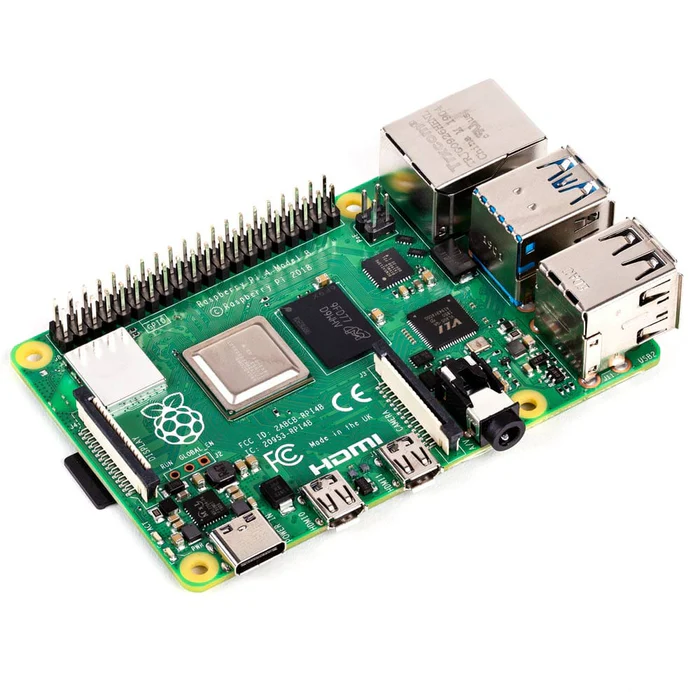
\includegraphics[width=.9\columnwidth]{figuras/rpi4.png}
    \caption{Raspberry Pi 4 Modelo B~\cite{rpi4}.}
    \label{fig:rpi4}
\end{figure}

\newpage

% Este documento \LaTeX~foi organizado em uma série de arquivos separados para cada Seção, localizados na pasta \texttt{editaveis}. 
% Confira ao longo dos arquivos como incluir
% figuras como a Fig. \ref{fig:rpi3}, além de tabelas, notas de rodapé e referências.
% Para acrescentar referências, altere o arquivo \texttt{editaveis/refs.bib}, que segue o formato BibTeX~\cite{ref:bibtex}. 

% Para manter o projeto organizado, acrescente suas figuras à pasta \texttt{figuras}. 
% % Confira no arquivo \texttt{editaveis/02\_introducao.tex} como incluir figuras como a Fig. \ref{fig:rpi3} e tabelas como a Tabela \ref{tab:pontuacao}.
% Para figuras e tabelas, não se preocupe com o posicionamento delas no texto. 
% O importante é que todas sejam referenciadas, assim como foi feito na segunda linha deste parágrafo.

% Todo o texto deve ser auto-contido; isto é, ele deve se explicar por si só. As figuras e tabelas somente \textit{auxiliam} no entendimento do texto. Sempre que o autor tiver que se explicar após a escrita, isto significa que o texto não está claro.

% O projeto completo deverá ser desenvolvido em ambiente Git público (GitHub, GitLab etc.), incluindo cronograma do projeto, código-fonte, código \LaTeX~deste relatório e resultados (planilhas, fotos etc).
% O repositório do projeto terá dois propósitos: servir de portfólio para os integrantes do grupo, e estender os conhecimentos de sala de aula para a comunidade em geral (créditos de extensão).



\section{Solução Proposta}
\subsection{Descrição de \textit{hardware}}\label{subsec:hardware}

Nesta Subseção, apresente as informações necessárias para se replicar o \textit{hardware} desenvolvido neste trabalho. 
Justifique suas escolhas, explicando tudo textualmente, e inclua:

\begin{itemize}
    \item Uma \textbf{lista de materiais} (BOM, do inglês \textit{bill of materials}) com os componentes necessários para a montagem do circuito~\cite{ref:bom}.
    \item Um \textbf{diagrama de blocos}, que fornece uma visão geral de como os circuitos discretos de um dispositivo ou sistema interagem. Os circuitos são representados por blocos, e suas relações são indicadas por linhas de interconexão, às vezes com setas~\cite{ref:blockdiagram}.
    \item Um ou mais \textbf{diagramas esquemáticos}, que incluem todos os componentes de um circuito, com cada componente tendo seu próprio símbolo específico~\cite{ref:esquematico}.
\end{itemize}
%A Tabela \ref{tab:BOM} e as Figuras \ref{fig:exemplo_diagrama} e \ref{fig:exemplo_esquem} apresentam exemplos de uma BOM, um diagrama de blocos e um esquemático correspondentes para um circuito conversor de corrente alternada para corrente direta.
A fim de obter uma solução mínima, todavia com todas as capacidades necessárias para concluir os objetivos traçados ao longo da introdução, o sensor BME280 foi escolhido com base em suas capacidades e o custo benefício apresentado.\\

%terminar de ler a específicação pra explicar isso aqui melhor
%eu quero conseguir basicamente afirmar que temos precisão 
% o suficiente pra duas casas decimais em booleano, que vai ser
% a precisão que o modelo de ia vai ser treinado em cima e vai 
% prover depois de treinado.
Após uma breve análise da específicação técnica do sensor, foi determinado que ele será capaz de operar nos ambientes propostos, bem como exposto ao ar livre sem apresentar riscos a sua operação. Capaz de comunicação por meio de protocolo I2C ou SPI, o sensor provê leituras de temperatura, umidade e pressão com resolução adequada ao conjunto de dados disponível em domínio público por meio do INMET\cite{inmet}, que disponibiliza suas leituras em ponto flutuante de 2 casas decimais. Ademais, o componente possui documentação suficiente na comunidade de usuários do Raspberry Pi para que seja possível o desenvolvimento do software sem a necessidade de manualmente escrever a interface, sendo meramente necessário conectar o sensor corretamente. \\

A fim de controlar o sensor, guardar leituras, calcular médias e executar um modelo de aprendizado de máquina, será utilizado o SoC Raspberry Pi 3 Model B (RPI3B) \cite{rpi3}, o qual, considerando que foi provido como empréstimo pela instituição, não aparecerá na BOM. O RPI3B possui um processador ARM com 4 núcleos, que serão utilizados para prover poder de multiprocessamento suficiente para sustentar uma solução de software que utilize largamente as capacidades do sistema simultaneamente possibilitando não necessitar de mais periféricos e possibilitando que o usuário utilize um aparelho celular ou computador para monitorar o funcionamento do sistema, contanto que tenha acesso à internet. Em outras palavras, a interface humano-computador será realizada por meio de um site. No mais, as necessidades de armazenamento do sistema são supridas facilmente por um cartão SD, o qual também foi obtido por meio de empréstimo com a instituição.\\

Em termos de memória provida pelo sistema, o SoC conta com 1Gb de RAM, suficiente para carregar um interpretador Python com modelos de análise computacional periodicamente para prover análises mais detalhadas da evolução da temperatura com o passar do tempo e/ou carregar o servidor, que será descrito em detalhes na seção de proposta de software.\\

%A proposta de uma estrutura física não é de grande importância, mas deve minimamente garantir que a leitura do sensor não será afetada pelo calor gerado pelo funcionamento do rpi3b e a integridade do sistema não será afetada pelo clima

A figura \ref{fig:exemplo_esquem} apresenta um esquemático de circuito de como a conexão foi realizada entre o SoC e o sensor e a tabela \ref{tab:BOM} apresenta a Lista de Materiais utilizada pelo projeto. 


%copiar e colar diagrama de blocos do datasheet do bme aqui.
%\begin{figure}[!htpb]
%\centering
%\includegraphics[width=.9\columnwidth]{figuras/Exemplo-diagrama-de-%blocos.png}
%\caption{Diagrama de blocos de exemplo: circuito conversor de corrente alternada para corrente direta~\cite{ref:block_n_schematic}.}
%\label{fig:exemplo_diagrama}
%\end{figure}

%Não temos um esquemático de circuito nos datasheets pro sensor
\begin{figure}[!htpb]
\centering
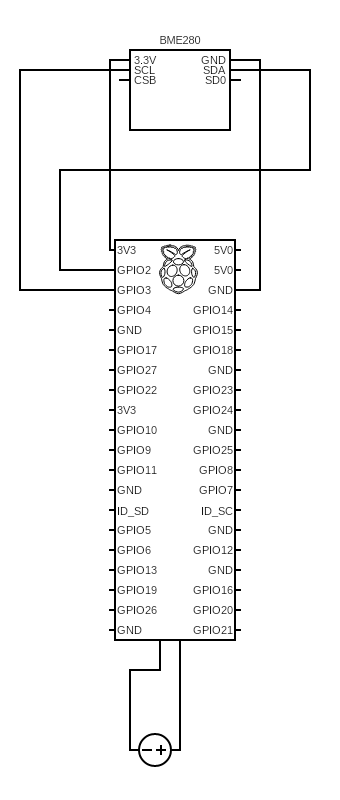
\includegraphics[width=.9\columnwidth]{figuras/circuit.png}
\caption{Esquemático de conexão do RPI3B com o sensor BME280}
\label{fig:exemplo_esquem}
\end{figure}

% A BOM tá basicamente feita se for só esse sensor até o final do projeto. 
\begin{table}[!htpb]
% increase table row spacing, adjust to taste
% \renewcommand{\arraystretch}{1.3}
\caption{Lista de materiais.}
\label{tab:BOM}
\centering
\begin{tabular}{ccc}
\hline
\textbf{Componente} & \textbf{Preço unitário} & \textbf{Quantidade}\\
\hline 
Módulo Sensor BME280 & R\$ 52,90 & 1 \\
Cabo Jumper Fêmea/Fêmea & R\$ 0,20 & 4 \\
\hline
\textbf{Total} & R\$ 53,70 & \\
\hline
\end{tabular}
\end{table}

Por fim, a Figura \ref{fig:diagramabloco} apresenta o diagrama de blocos do sistema, representando os principais componentes de hardware que serão utilizados para correto e completo funcionamento.

%had to do this atrocity with the height so it would fit 
\begin{figure}[!ht]
\centering
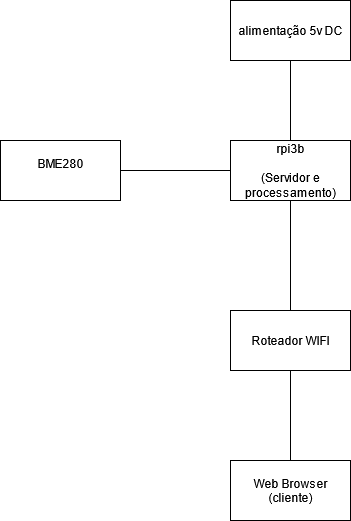
\includegraphics[width=.7\columnwidth]{figuras/diagramabloco.png}
\caption{Diagrama de blocos do sistema proposto}
\label{fig:diagramabloco}
\end{figure}

%Tópicos importantes a serem descritos nesta Subseção incluem:

%\begin{itemize}
%    \item \textbf{Processamento:} RPi 3, Arduino, MSP430 etc.
%    \item \textbf{Sensores:} tipos (temperatura, pressão etc.), taxas de amostragem e precisões necessárias;
%    \item \textbf{Atuadores:} motores DC, relés, LEDs etc.
%    \item \textbf{Comunicações:} UART, I2C, SPI, USB, WiFi, Bluetooth etc.
%    \item \textbf{Armazenamento:} \textit{hard drive}, cartão SD, \textit{pendrive} etc.
%    \item \textbf{Interfaces com o usuário:} botões, LEDs, display, touchscreen etc.	
%    \item \textbf{Estrutura física:} formato, dimensões, posicionamento dos circuitos, dos sensores, dos atuadores e da interface com o usuário.
%\end{itemize}

\subsection{Descrição de \textit{software}}\label{subsec:software}

\begin{figure*}[!htpb]
\centering
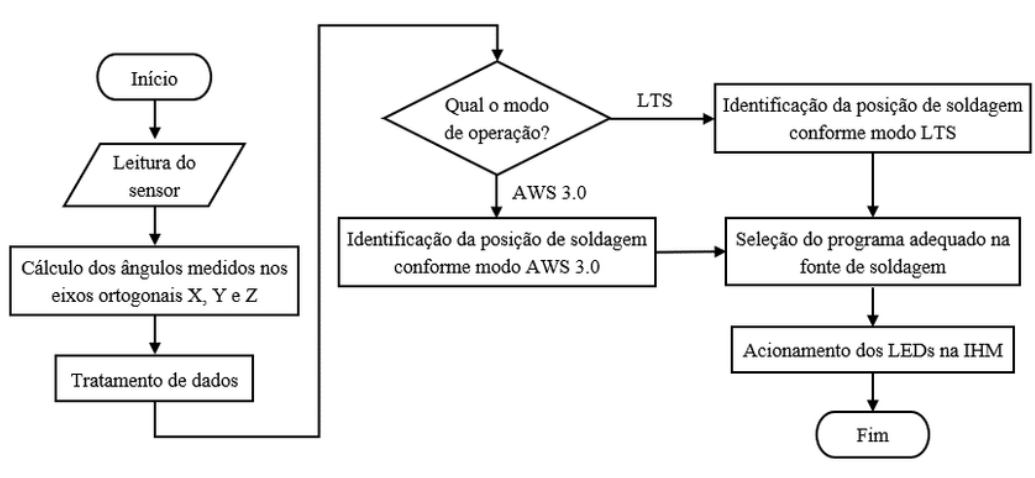
\includegraphics[width=.8\textwidth]{figuras/exemplo_de_fluxograma.png}
\caption{Exemplo de fluxograma~\cite{ref:exemplo_fluxograma}.}
\label{fig:exemplo_fluxograma}
\end{figure*}

Explique textualmente o algoritmo desenvolvido.
Esta subseção do relatório \textbf{NÃO CONSISTE} em simplesmente replicar o código, e sim em explicar como ele funciona, justificando suas escolhas de projeto.
O código pode ser apresentado como um apêndice ao relatório. 

Utilize fluxogramas como o da Fig. \ref{fig:exemplo_fluxograma} para auxiliar no entendimento do algoritmo desenvolvido.
Repare que a figura ocupa as duas colunas, usando o comando \verb|\begin{figure*} \end{figure*}| ao invés de \verb|\begin{figure} \end{figure}|.

Tópicos importantes a serem descritos nesta Subseção incluem:

\begin{itemize}
    \item \textbf{Coleta de dados:} conexão com sensores, definição da taxa de amostragem etc.
    \item \textbf{Processamento de dados:} filtro média-móvel, detecção de faces, reconhecimento de caracteres etc.	
    \item \textbf{Atuadores:} PWM, escrita em \textit{drivers} etc.	
    \item \textbf{Armazenamento/transmissão:} salvar em arquivo, enviar para a nuvem etc.	
    \item \textbf{Interface com o usuário:} GUI, interrupções para botões etc.
    \item \textbf{Inserção do programa no sistema operacional:} inicialização automática (\textit{crontab}, \texttt{/etc/init.d}), desligamento de serviços desnecessários, \textit{Buildroot} etc.
\end{itemize}
\section{Resultados Experimentais}\label{sec:resultados}

Os experimentos deverão validar o funcionamento do protótipo desenvolvido, comparando o que se espera dele com o que foi possível alcançar.
Explique os experimentos definidos, seguido de uma análise crítica dos resultados esperados e obtidos.
Em caso de divergências, aponte as possíveis causas. 
Explique claramente tudo o que foi feito.

Serão esperados os seguintes resultados para cada ponto de controle:

\begin{itemize}
    \item \textbf{PC1:} proposta do projeto, sem resultados práticos;
    \item \textbf{PC2:} funcionamento básico de cada parte fundamental, mostrando com quaisquer linguagens de programação que é possível conectar estas partes ao Raspberry Pi;
    \item \textbf{PC3:} refinamento do protótipo em linguagem C/C++;
    \item \textbf{PC4:} refinamento do protótipo em linguagem C/C++.
\end{itemize}
Fazendo uma analogia do projeto com a montagem de um quebra-cabeças, o PC1 corresponderia à escolha do quebra-cabeças, o PC2 seria a disposição de todas as peças sobre a mesa, e os PCs 3 e 4 seriam a montagem do quebra-cabeças.


A partir do PC2, os grupos deverão apresentar em sala de aula o funcionamento atualizado do sistema, e aproveitar os resultados documentados nos PCs para compôr esta Seção na entrega final.
Desta maneira, os pontos de controle indicam com clareza se o trabalho do grupo está adiantado ou atrasado em relação à Entrega Final\footnote{Desenvolvendo bem os quatro PCs, o grupo poderá chegar à entrega final com pouco trabalho por fazer.}.

A Tabela \ref{tab:pontuacao} apresenta a pontuação dada a cada uma das Seções e Subseções na avaliação final deste trabalho, bem como os pontos de controle onde elas serão pré-avaliadas.

\begin{table}[!htpb]
% increase table row spacing, adjust to taste
\renewcommand{\arraystretch}{1.3}
\caption{Avaliações deste trabalho}
\label{tab:pontuacao}
\centering
\begin{tabular}{ccc}
\hline
\textbf{Seção} & \textbf{Pontuação final} & \textbf{Pré-avaliação} \\
\hline 
\textit{Abstract} & 1 & ---\\
\ref{sec:intro}. Introdução & 1 & PC1 \\
\ref{subsec:hardware}. \textit{Descrição de} Hardware & 2 & PC2, PC3 e PC4\\
\ref{subsec:software}. \textit{Descrição de} Software & 3 & PC2, PC3 e PC4\\
\ref{sec:resultados}. \textit{Resultados Experimentais} & 2 & PC2, PC3 e PC4 \\
\ref{sec:conclusoes}. \textit{Conclusões} & 1 & --- \\
\hline
\textbf{Total} & 10 \\
\hline
\end{tabular}
\end{table}
\section{Conclusões}\label{sec:conclusoes}

Retome sucintamente os principais pontos do relatório: descrição do problema, solução utilizada e resultados obtidos.  Em seguida, revise o que se pôde aprender com este projeto, e apresente passos futuros.			


% \section*{Agradecimentos}

% \textbf{Esta seção não é obrigatória.} Ela é importante quando se deseja reconhecer o trabalho de alguém que não participou diretamente do trabalho desenvolvido, mas que teve papel importante. Os autores gostariam de agradecer...

\bibliographystyle{IEEEtran}
\bibliography{editaveis/refs}
\section*{Apêndice}

\textbf{Esta seção não é obrigatória.} Apêndices e anexos são materiais complementares ao texto que só devem ser incluídos quando forem imprescindíveis à compreensão deste:

\begin{itemize}
    \item Apêndices são textos elaborados pelo autor a fim de complementar sua argumentação.
    \item Anexos são os documentos não elaborados pelo autor, que servem de fundamentação, comprovação ou ilustração, como mapas, leis, estatutos etc.

\end{itemize}





% trigger a \newpage just before the given reference
% number - used to balance the columns on the last page
% adjust value as needed - may need to be readjusted if
% the document is modified later
%\IEEEtriggeratref{8}
% The "triggered" command can be changed if desired:
%\IEEEtriggercmd{\enlargethispage{-5in}}

% references section

% can use a bibliography generated by BibTeX as a .bbl file
% BibTeX documentation can be easily obtained at:
% http://www.ctan.org/tex-archive/biblio/bibtex/contrib/doc/
% The IEEEtran BibTeX style support page is at:
% http://www.michaelshell.org/tex/ieeetran/bibtex/
%\bibliographystyle{IEEEtran}
% argument is your BibTeX string definitions and bibliography database(s)
%\bibliography{IEEEabrv,../bib/paper}
%
% <OR> manually copy in the resultant .bbl file
% set second argument of \begin to the number of references
% (used to reserve space for the reference number labels box)
% \begin{thebibliography}{100}

% \bibitem{ref:rpi3}

% \bibitem{IEEEhowto:kopka}
% H.~Kopka and P.~W. Daly, \emph{A Guide to \LaTeX}, 3rd~ed.\hskip 1em plus
%   0.5em minus 0.4em\relax Harlow, England: Addison-Wesley, 1999.

% \end{thebibliography}




% that's all folks
\end{document}


